\subsection{Results of the new mechanism tests}
The second study adds 732 model-based missions, including the pilot and declared diagnostics. Reciprocal versus periodic handover changes coverage by -0.21 [-0.35, -0.09] percentage points and total energy by -5.55 Wh. Relative to greedy handover the coverage contrast is -0.45 [-0.63, -0.28] points. Nonlinear versus linear inhibition changes coverage by +0.01 [-0.04, +0.06] points and energy by -1.48 Wh. Brackets are paired 95\% bootstrap intervals, not predictive bounds for a new vessel platform.
\begin{table}[t]\centering\small
\caption{New main-study means. Each policy has 96 missions across two radio profiles and four scenarios.}
\begin{tabular}{lrrr}\toprule Policy & $\bar C$ & $E$ [Wh] & AoI [s]\\\midrule
Economic & 0.6957 & 300.9 & 49.3 \\
Periodic handover & 0.6843 & 280.1 & 51.0 \\
Greedy handover & 0.6867 & 282.9 & 50.6 \\
Reciprocal handover & 0.6822 & 274.5 & 51.2 \\
Linear inhibition & 0.6962 & 301.0 & 49.4 \\
Nonlinear inhibition & 0.6963 & 299.5 & 49.3 \\
\bottomrule\end{tabular}\label{tab:v4means}\end{table}
\begin{figure*}[tbp]\centering
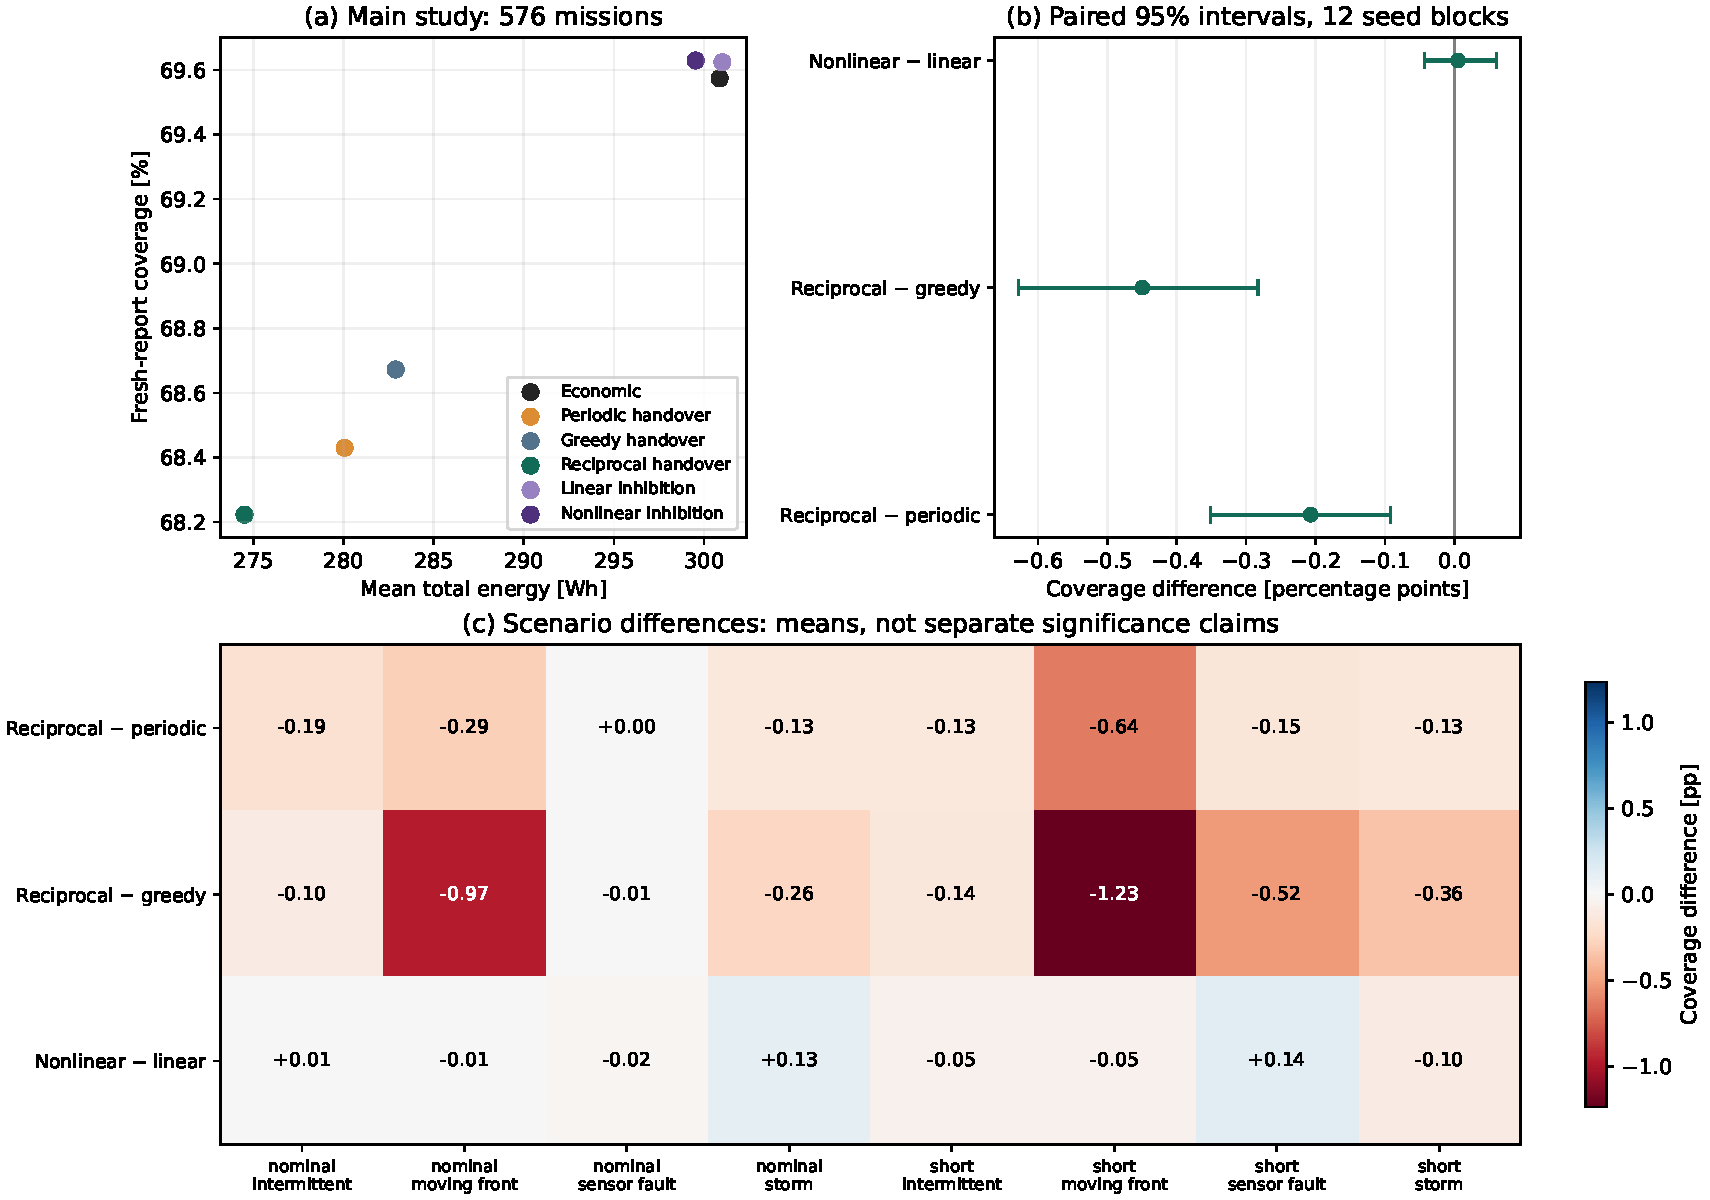
\includegraphics[width=.97\textwidth]{figures/bio_mechanisms.pdf}
\caption{Additional biological mechanisms with matched restrictions. Main-study coverage--energy means, paired coverage contrasts, and scenario-specific differences. A reduced movement budget can save energy while losing timely monitoring.}
\label{fig:v4bio}\end{figure*}
\begin{table*}[tbp]\centering\small
\caption{Prespecified new biological contrasts and small diagnostics. Coverage differences are in percentage points, with paired 95\% intervals. Main $p_H$ values apply Holm adjustment to three coverage tests; diagnostics are descriptive.}
\begin{tabular}{llrrr}\toprule Setting & Contrast & $\Delta C$ [95\% interval] & $\Delta E$ [Wh] & $p_H$\\\midrule
Main, 12 blocks & Reciprocal -- periodic & -0.21 [-0.35, -0.09] & -5.55 & 0.008 \\
Main, 12 blocks & Reciprocal -- greedy & -0.45 [-0.63, -0.28] & -8.38 & 0.002 \\
Main, 12 blocks & Nonlinear -- linear & +0.01 [-0.04, +0.06] & -1.48 & 0.850 \\
Shifted, 4 blocks & Reciprocal -- periodic & -0.28 [-0.59, +0.04] & -3.28 & -- \\
Shifted, 4 blocks & Reciprocal -- greedy & -0.36 [-0.67, -0.16] & -5.35 & -- \\
Shifted, 4 blocks & Nonlinear -- linear & -0.07 [-0.14, -0.00] & +0.46 & -- \\
128 paths, 4 blocks & Reciprocal -- periodic & +0.03 [-0.41, +0.47] & -6.16 & -- \\
128 paths, 4 blocks & Reciprocal -- greedy & -0.58 [-0.74, -0.42] & -6.32 & -- \\
128 paths, 4 blocks & Nonlinear -- linear & -0.01 [-0.21, +0.18] & +0.33 & -- \\
\bottomrule\end{tabular}\label{tab:v4contrasts}\end{table*}
These adaptations should be judged against their matched controls and against unrestricted economic control. Reciprocal handover versus economic control changes coverage by -1.35 [-1.60, -1.13] points; nonlinear inhibition versus economic control changes it by +0.06 [-0.03, +0.16] points. A small main-study contrast alone does not establish a generally useful biological advantage. The changed observation law and integration resolution are particularly relevant because all policies still optimize a sampled, imperfect prospective score.
